%%%%%%%%%%%%%%%%%%%%%%%%%%%%%%%%%%%%%%%%%%%%%%%%%%%%%%%%%%%%%%%%%%%%%%%%%%%%%%%%
\chapter{Terminology}
%%%%%%%%%%%%%%%%%%%%%%%%%%%%%%%%%%%%%%%%%%%%%%%%%%%%%%%%%%%%%%%%%%%%%%%%%%%%%%%%

In this chapter we define certain terms that have specific meanings in the context of Landslide.

\section{Basic Terms}

\begin{enumerate}
	\item {\bf Guest kernel}:
		The kernel which is being tested for concurrency bugs by Landslide.
	\item {\bf Test case}:
		Abstractly, the set of inputs under which the guest kernel is tested. Practically, a user-space program which runs on top of the guest kernel to execute a particular set of system calls, while Landslide performs systematic exploration.
		\revision{The expected results of the test case's system call invocation pattern informally define the kernel specification.}
\suspend{enumerate}

\section{Scheduling Terms}

\revision{The following terms refer to parts of the guest kernel's execution.}

\resume{enumerate}
	\item {\bf Thread}:
		One participating agent in a concurrent program, which executes code sequentially, with the potential to be interleaved with the execution of other threads in the system.
		Each thread has a unique numeric identifier (TID).
	\item {\bf Involuntary preemption}:
		A context switch from one thread to another caused by a nondeterministic event, such as a timer tick or device interrupt. The systematic testing framework must control all sources of nondeterminism. In this work, we focus only on timer-driven thread switches.
	\item {\bf Voluntary reschedule}:
		A context switch from one thread to another which the guest kernel performed automatically, not triggered by nondeterministic events and/or Landslide but rather as part of its normal execution.\footnote{Voluntary reschedules may or may not be necessary for the kernel to behave correctly at all (for example: switching away from an exiting thread or from a thread blocked on \texttt{wait} is necessary, but switching to a newly-forked thread is not). Involuntary preemptions are never necessary for correct kernel behaviour.}
		See Section~\ref{sec:components-arbiter}.
\suspend{enumerate}

\section{Systematic Exploration Terms}

\begin{figure}[h]
	\centering
	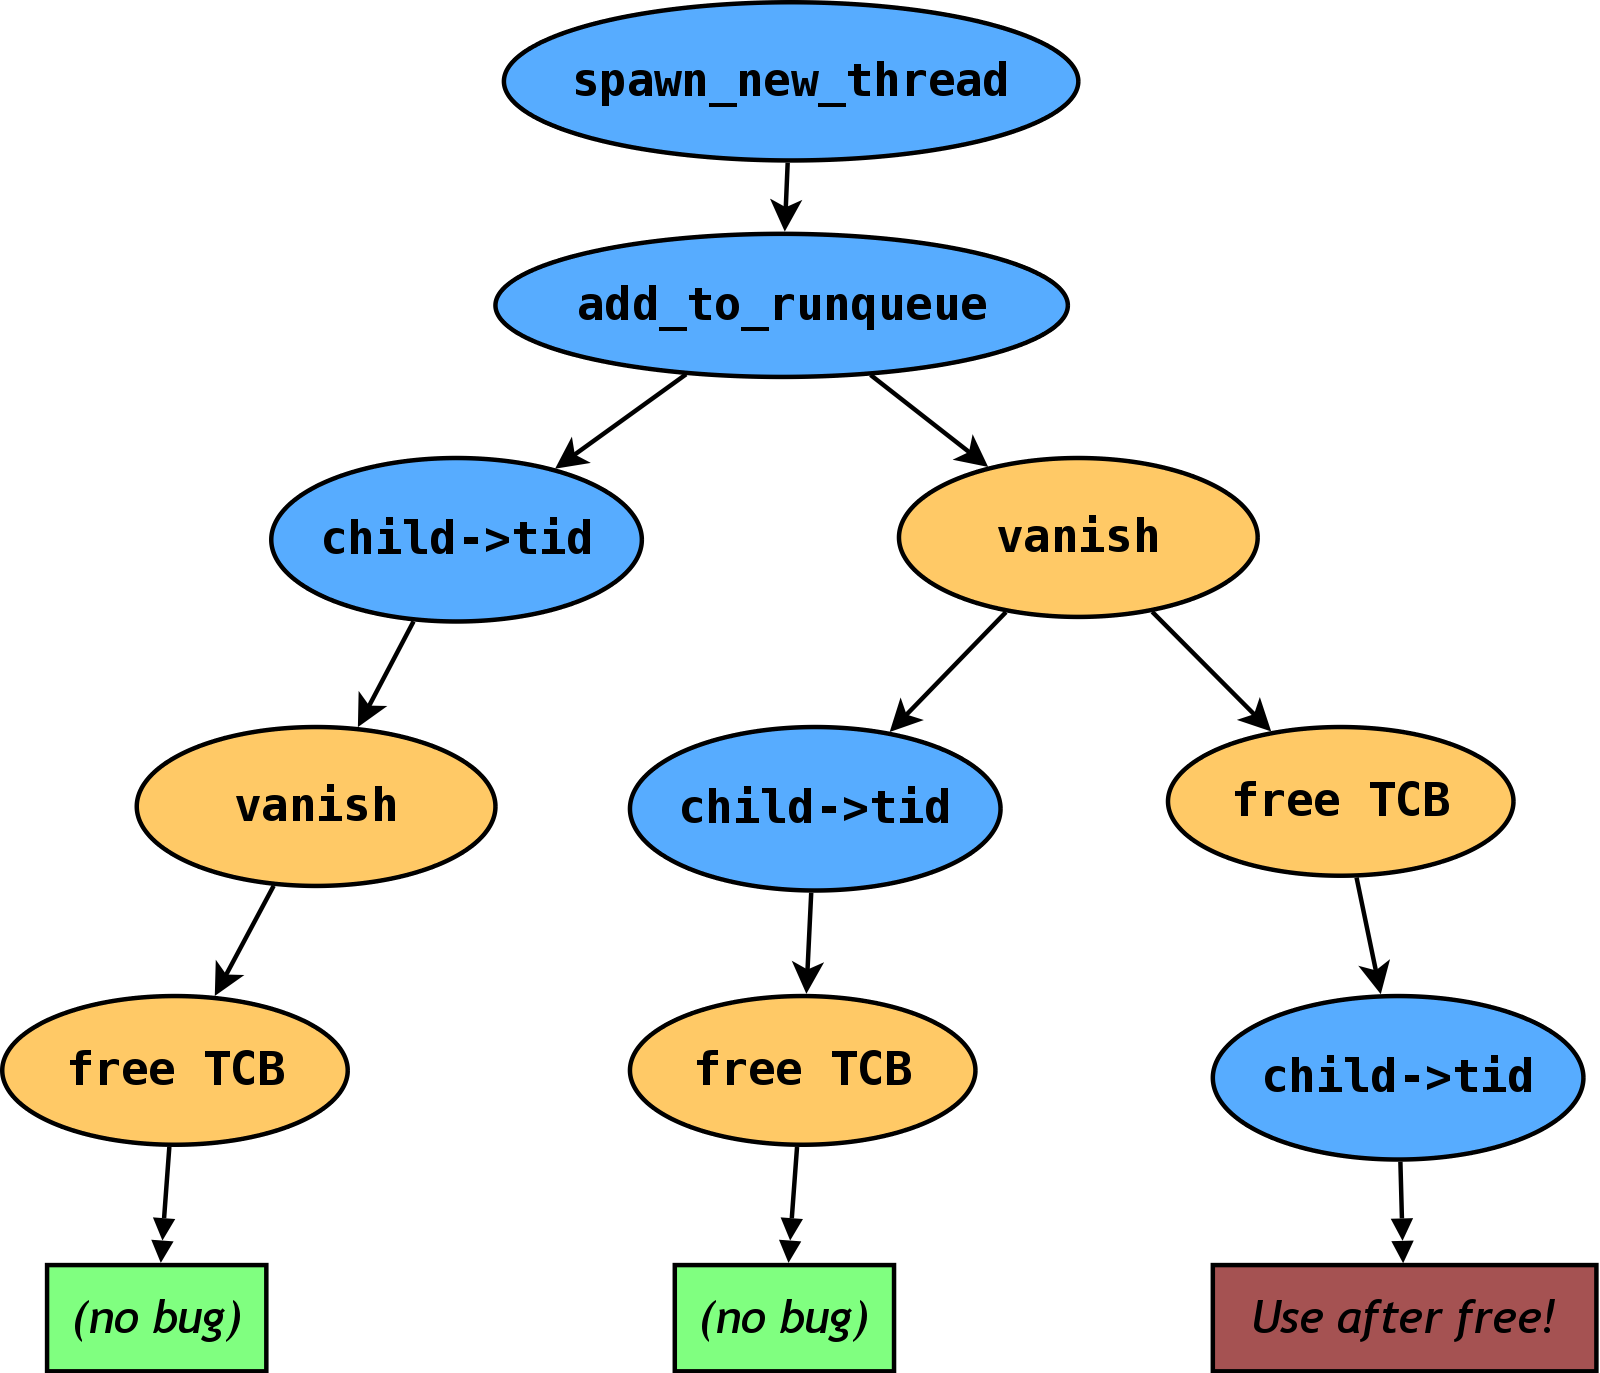
\includegraphics[width=0.75\textwidth]{threadfork.png}
	% TODO: make some other subfigs
	\caption{A simple decision tree, showing possible interleavings of a buggy \texttt{thread\_fork} implementation. (This describes a bug studied in Section~\ref{sec:eval-thread-fork}.)}
	\label{fig:threadfork}
\end{figure}

\revision{The following terms refer to parts of Landslide's analysis, regardless of the kernel under test's implementation.}

\resume{enumerate}
	\item {\bf Decision point}:
		A point during execution (between two consecutive instructions, precisely) which is deemed ``interesting'' in terms of the likelihood that thread switches at that point will cause concurrency bugs to arise. Every thread switch occurs at a decision point; some are voluntary reschedules caused by the kernel and others are involuntary preemptions caused by Landslide.
	\item {\bf Transition}:
		A sequence of instructions executed by a single thread between two decision points. At a given decision point, Landslide chooses which thread will run (and causes it to do so), and that thread executes a transition, after which point Landslide will have identified a subsequent decision point
	\item {\bf Decision set} (or {\bf Set of decision points}):
		One or more predicates on the execution state of the guest kernel which identify whether any current state should be a decision point. (For example, when we say ``the decision set including all calls to \texttt{mutex\_lock}'', the corresponding predicate is simply ``did the kernel just invoke \texttt{mutex\_lock}?''.)
	\item {\bf Decision tree} (or {\bf Execution tree}):
		The tree defined by the possibility at each decision point of causing any runnable thread to execute its own transition. Abstractly, this tree comprises all possible states reachable by any interleaving of threads.
		A decision tree is created/discovered during an exploration using a particular decision point set; the set is what the user configures, and the tree is what arises as a result.
	\item {\bf Branch}:
		One particular execution of the test case; a set of decision points with exactly one transition between each of them, characterising a single interleaving of threads.
	\item {\bf Interleaving}:
		A less precise / more abstract term for a branch, or for a subset of transitions which make up a branch.
	\item {\bf Bug}: An execution state which Landslide identifies as incorrect, which is indicative of illegal behaviour. Each branch of the tree may or may not have a bug in it. See Section~\ref{sec:techniques-bugs}.
	\item {\bf Backtracking}:
		Performed at the end of each branch of the tree, when the test case has finished running. Landslide identifies a decision point from the current branch at which the \revision{next interleaving to explore diverges from the current one}, reverts the state of the guest kernel to what it was at that decision point, and causes a different thread to run, hence exploring a different branch/interleaving.
	\item {\bf Decision trace}:
		A list of information about all decision points in a given branch, printed when a bug is found to help the user analyse its cause. Contains, for each decision point, the TID of the thread that was running previously, the TID that was newly chosen, the current instruction pointer, and the stack trace of the previous thread at the point it was switched away from.\footnote{Though Landslide does not provide it, a decision trace may also contain for each transition a list of shared memory accesses that conflicted with other transitions, and/or a listing of happens-before relationships between transitions.}
\end{enumerate}

% vim: ft=tex
